\section{System's Perspective}

\subsection{Design and Architecture of MiniTwit}
The MiniTwit application architecture has been designed by following some important software design guidelines 
such as low coupling, high cohesion, and the Single Responsibility Principle(SRP). 
These concepts are closely related and basing the development on those helped us create software that is easier to work with. 

The SRP states that each part of a software system should be responsible for one thing and therefore only have one reason to change(KILDE). 
Cohesion is closely related to the SRP and it is a measure of the degree to which related functionality is grouped together in a single coherent unit(KILDE). 
In general, the goal is to have modules with high cohesion as this ensures that the code in a given module is focused on a single aspect of the application's functionality. 
This is important as having too much functionality in a single module is likely to result in code that is hard to both understand and change. 

Finally, coupling refers to the degree of interdependence between the modules within a system and it measures how well-defined the boundaries between different modules are. 
Coupling can be classified as either low or high and low coupling implies that modules' knowledge of other modules' internal implementation details have been minimized(KILDE).
Together the SRP, low coupling, and high cohesion are key enablers when it comes to reducing complexity and thereby ensuring a strong foundation for designing extendable software. \\

To achieve low coupling and high cohesion the MiniTwit application has been split into three layers namely persistence, web, and application as seen in figure \ref{fig:minitwit}. 
As prescribed by the SRP each layer is responsible for one thing and we have minimized the dependencies between the layers thus making it easier to extend MiniTwit with new features. 
It also reduces cognitive load as it makes it easier to navigate the system because code related to the same functionality is grouped together. 


% Fix system architecture image.
\begin{figure}[H]
    \centering
    \captionsetup{justification=centering,margin=1cm}
    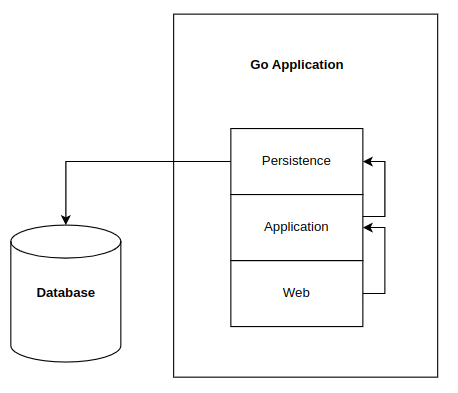
\includegraphics[width=0.8\linewidth]{./images/system_architecture.png}
    \caption{MiniTwit Architecture}
    \label{fig:minitwit}
\end{figure}



\subsubsection{Application, Persistence, and Web}
In the application layer, all code related to core business logic is found. This includes the models that MiniTwit is built upon such as User and Message. 
Business logic has been separated from other parts of the application as doing so allows developers to understand and 
modify business logic without impacting other components of the application. Secondly, separating business logic promotes reusability, 
as the code can easily be shared across different parts of the application.     \\

In the persistence layer, the database setup is configured. We use an Object Relational Mapper(ORM) called GORM to interact 
with the database as it abstracts some of the complexity that comes with a relational database(Link to ORM section). 
Migrations and data seed are also handled in the persistence layer the latter only when the database contains no data. 
This is useful for local development and in test environments as the application can be tested without having to create users first. \\

The web layer is implemented using a lightweight Go web framework called Gin. 
Gin was chosen because it offers a minimalistic and fast approach to building web applications as it provides 
essential features like routing, middleware support, JSON handling, and request/response binding(KILDE). 
All features that would have taken a long time to implement from scratch. Gin route requests to controllers 
which coordinate the request/response cycle which includes ensuring the validity of a given request. 
Some requests include new data such as tweets and this data is used to update the database state after 
which HTML containing the updated state is generated and returned to the client. 


\subsection{Dependencies of MiniTwit system}

For the MiniTwit application to run we are depending on first and foremost Digital Ocean whos servers the application is 
hosted on. The servers are running 9 docker containers responsible for: 
\begin{itemize}
    \item The Database running on a postgres:14.1-alpine image - Responsible for holding all the users data.
    \item The Server itself running on a golang:bullseye image.
    \item A redis server for storing sessions and the integer 'latest'.
    \item Elastic Search - Indexing logs such that we can search and analyse them
    \item Filebeat for collecting and forwarding the logging to Elastic search
    \item Kibana for visualizing the results from Elastic search
    \item Prometheus for monitoring the application in terms of CPU usage and request time
    \item Grafana for visualizing the monitoring
    \item Nginx for load balancing the incoming traffic to the different services
\end{itemize}

From within each of these containers we depend on large number of libraries of which the major ones we consider to be:
\begin{itemize}
    \item Gorm used for object-relational mapping allowing us to perform CRUD operations io GO.
    \item Gin handling all of the routing of the HTTP methods.
    \item x/crypto/bcrypt library for hashing the user password.
\end{itemize}

For initializing the containers we used docker-compose and docker swarm. Hence we also depend on docker, docker-compose
and terraform which was used to init all the servers
\begin{itemize}
    \item connect to docker swarm nodes via token
    \item manage ssh keys on nodes 
    \item mange config an secret on notes
\end{itemize}

In a more board sense the application also depend on Go, Ubuntu, python and SSH protocol to work. At last we 
also depend on pre-build git workflows such as \textit{docker/build-push-action@v2} or \textit{rymndhng/release-on-push-action@master}.

%OBS MSc students: Remember to log and provide good arguments for the choice of programming language and framework
\subsubsection{Arguments for programming language and framework}
We initially set out to use FastAPI in Python, but eventually settled on GO for multiple reasons. From a personal 
development perspective, learning a new language is rarely a poor choice. Go is well-known for being relatively 
fast to learn, whilst maintaining speed. From a more technical perspective Go has advantages over many languages. 
It's fast, it has concurrency built-in, and it has a strong standard library support, with most important features, 
even templating, being available as a standard package.\\

Gin is not the fastest Go framework, but it has several advantages. It is well-maintained, has over twice the 
amount of github stars than the next most popular framework, and is one of the faster go web frameworks.\\

Whilst implementing the application in fastAPI might have been faster and easier, due to both prior python 
knowledge, and general simplicity, the advantages of using go with the GIN framework can't be overstated. 

%OBS MSc students: Remember to log and provide good arguments for the choice of virtualization techniques and deployment targets
\subsubsection{Arguments for virtualization techniques and deployment targets}
Docker was chosen because it's the industry standard. Other container strategies are good, but given knowledge 
of future need for orchestration (in either docker swarm or kubernetes) Docker was an obvious choice.\\

We used Digital Ocean mainly for budgetary reasons and for ease of deployment. Using the Github Student 
Starter pack, \$200 in free credits were made available to us. This was enough to ensure that the application 
was able to run for the duration of the course. In fact it allowed us to test out the different deployment strategies
from monoroid and containerized application being spin up with only docker-compose to more advanced strategies such as
running on multiple servers with services running to mimimize downtime.\\

Using multiple accounts furthermore allowed us to create a parallel Digital ocean was employed for budgetary reasons, and also because the guides were made for it.
It's also more accessible than other more complicated providers such as AWS. 

\subsubsection{Arguments for ORM and DBMS}
%OBS MSc students: Remember to log and provide good arguments for the choice of ORM framework and chosen DBMS.
In regards to choosing ORM(Object-relational mapping) and DBMS(Database Management Systems) we settled on 
using \textit{PostgresSQL} as our DBMS and \textit{Gorm} for ORM. In terms of choosing DBMS we considered 
\textit{SQLite} and \textit{digital ocean manged db}:
\begin{itemize}
    \item Potential arguments over SQLite 
    \begin{itemize}
        \item Scalability
        \item Concurrency
        \item No user management
        \item Network access        
    \end{itemize}
    \item Potential arguments over e.g. digital ocean manged db
    \begin{itemize}
        \item Cost
    \end{itemize}
\end{itemize}

For ORM we considered \textit{XORM} and \textit{beego} but due to our limited experience with GO we choose Gorm 
since it widely used, well documented and has better superior features like sanitizing input \footnote{\url{https://blog.logrocket.com/comparing-orm-packages-go/ & https://sumit-agarwal.medium.com/gorm-vs-xorm-part-1-d156ba9de404}}.


\subsubsection{Arguments for Terraform}
% Argue for Terraform choice??
- Infrastructure as code is important for maintainability reasons. Therefore Terraform was an obvious choice.
Terraform is for remote cloud providers. Vagrant is for local development. 

\subsection{Important Interactions of Subsystems}
In the image below the interactions between our subsystems can be seen:

\begin{figure}[H]
    \centering
    \captionsetup{justification=centering,margin=1cm}
    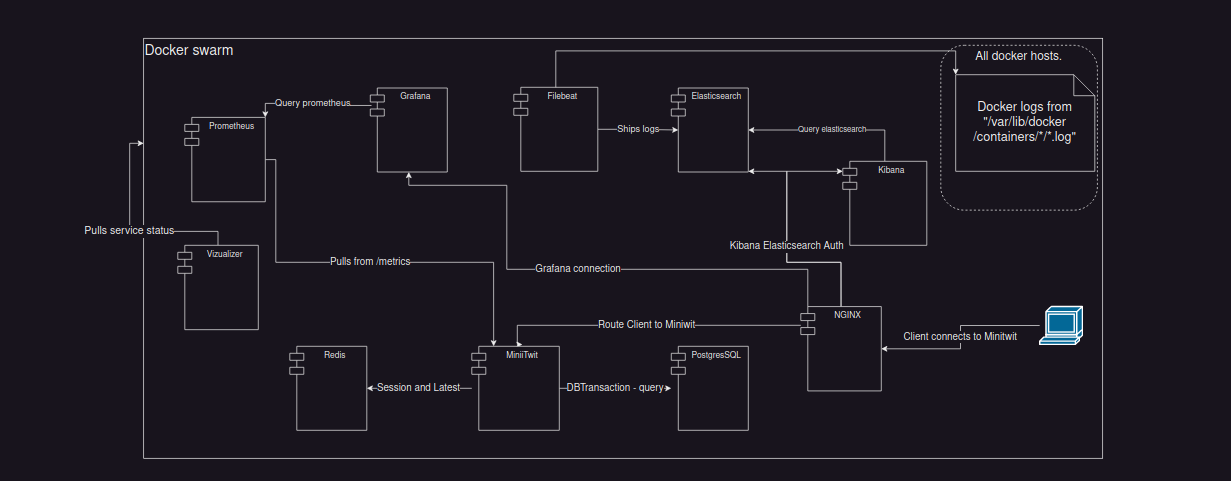
\includegraphics[width=0.8\linewidth]{report/images/InteractionsOfSystems.png}
    \caption{Subsystem interactions}
    \label{fig:minitwit}
\end{figure}

\subsection{Current state of the system}
In the current state of the system our stack consists of: 
\begin{itemize}
    \item Application running on Digital Ocean
    \item Run tests in CI/CD pipeline within an isolated environment
    \item Monitoring the application with Prometheus and Grafana
    \item Code quality checks using Golangci-lint in the CI/CD pipeline checking for typecheck, gosimple, unused etc.
    \item Logging using elastic search and Kibana
\end{itemize}
We did not manage to get Docker swarm and Redis up and running. Docker swarm were missing to be setup 
in our CI/CD chain and Redis seemed to be running locally but a bug on prod seemed to ruin Redis.

\subsection{Project License}
